\documentclass[conference]{IEEEtran}
\IEEEoverridecommandlockouts
\usepackage{cite}
\usepackage{amsmath,amssymb,amsfonts}
\usepackage{graphicx}
\usepackage{textcomp}
\usepackage{xcolor}
\usepackage[utf8]{inputenc}
\usepackage[spanish,es-nodecimaldot]{babel}
\addto\captionsspanish{\renewcommand{\tablename}{Tabla}}
\addto\captionsspanish{\renewcommand{\figurename}{Fig.}}
\usepackage{hyperref}
\usepackage{booktabs}
\usepackage{url}
\usepackage{listings}
\usepackage{placeins}
\usepackage{tikz}
\usetikzlibrary{shapes.geometric, arrows.meta, positioning, fit, backgrounds}

\lstset{
  basicstyle=\ttfamily\scriptsize,
  breaklines=true,
  columns=fullflexible,
  frame=single,
  backgroundcolor=\color{black!3},
  numbers=left,
  numberstyle=\tiny\color{gray},
  showstringspaces=false,
  captionpos=b,
  xleftmargin=1.2em,
  framexleftmargin=1em
}

\begin{document}

\title{Prueba de esfuerzo de un sistema Asterisk:\\
aplicaci\'on de \textit{Load}, \textit{Stress} y \textit{Spike Testing} sobre AGI--TAXI\\
{\footnotesize \textsuperscript{*}Informe Final --- Seminario de Voz IP, Universidad de Antioquia, 2026}
}

\author{
\IEEEauthorblockN{Ana Mar\'ia Garz\'on}
\IEEEauthorblockA{\textit{Facultad de Ingenier\'ia} \\
\textit{Universidad de Antioquia}\\
Medell\'in, Colombia}
\and
\IEEEauthorblockN{Juan Esteban Cardozo Rivera}
\IEEEauthorblockA{\textit{Facultad de Ingenier\'ia} \\
\textit{Universidad de Antioquia}\\
Medell\'in, Colombia \\
juan.cardozor@udea.edu.co}
\and
\IEEEauthorblockN{V\'ictor Manuel Restrepo}
\IEEEauthorblockA{\textit{Facultad de Ingenier\'ia} \\
\textit{Universidad de Antioquia}\\
Medell\'in, Colombia}
}

\maketitle

\begin{abstract}
La capacidad operativa de un PBX basado en Asterisk se ve limitada por
el procesamiento de se\~nalizaci\'on SIP, el manejo de canales RTP y la
l\'ogica de negocio invocada por las extensiones. Este informe final
del proyecto de prueba de esfuerzo del Seminario de Voz IP --- que
consolida y extiende lo entregado en las Entregas 1 y 2 ---
caracteriza el sistema AGI--TAXI (Asterisk 20.19 sobre Debian Trixie)
mediante la aplicaci\'on de tres de las cinco t\'ecnicas de
\textit{stress testing} descritas en el marco te\'orico: \textit{Load
Testing} (rampa controlada 10--300 concurrentes en dos escenarios
pareados Echo vs AGI), \textit{Stress Testing} (rampa extendida
400--1500 concurrentes para buscar el punto de quiebre) y
\textit{Spike Testing} (patr\'on baseline / pico 15$\times$ /
recuperaci\'on). Sobre el escenario sin RTP se procesaron en total
m\'as de 88\,000 llamadas SIP con tasa de \'exito del 100\,\% y consumo
de CPU pico de 29\,\%, lo que permite concluir que la pila PJSIP de la
VM tiene un margen muy superior al previsto inicialmente. Se incluyen
pantallazos directos de los archivos de configuraci\'on, de la
verificaci\'on en l\'inea de comandos de Asterisk, de SIPp en
ejecuci\'on y de los res\'umenes finales como evidencia de cada fase
del experimento. La trazabilidad queda garantizada mediante archivos
de configuraci\'on, escenarios XML, scripts de monitoreo y CSVs de
evidencia publicados en el repositorio del proyecto.
\end{abstract}

\begin{IEEEkeywords}
Asterisk, SIPp, VoIP, load testing, stress testing, PJSIP, AGI
\end{IEEEkeywords}

\section{Introducci\'on}

En la Entrega 1 del proyecto se describieron las cinco t\'ecnicas de
\textit{stress testing} aplicables a un PBX Asterisk ---
\textit{Load Testing}, \textit{Stress Testing}, \textit{Spike Testing},
\textit{Soak Testing} y \textit{Codec Stress Testing} ---, las
m\'etricas relevantes (CPU, CPS, llamadas concurrentes, jitter,
p\'erdida de paquetes, latencia y MOS) y las herramientas para llevarlas
a cabo, con SIPp \cite{ref_sipp} como n\'ucleo del proceso. En la
Entrega 2 se materializ\'o ese marco te\'orico con la primera de las
cinco t\'ecnicas, \textit{Load Testing}, sobre el sistema AGI--TAXI
\cite{ref_agitaxi}. El presente informe final consolida ambos
documentos y a\~nade las evidencias de aplicaci\'on de dos t\'ecnicas
adicionales --- \textit{Stress Testing} y \textit{Spike Testing} ---
sobre la misma VM, cubriendo as\'i tres de las cinco t\'ecnicas
descritas, conforme al requisito de la Entrega Final del seminario.

El objetivo es responder, sobre la VM del proyecto, tres preguntas
operativas complementarias: \textit{(i) cu\'antas llamadas
concurrentes puede sostener el PBX en r\'egimen normal manteniendo un
consumo de CPU inferior al 80\,\% y un porcentaje de llamadas exitosas
superior al 99\,\%} (zona de operaci\'on); \textit{(ii) cu\'al es el
punto de quiebre del sistema cuando se le exige por encima de su
capacidad esperada} (l\'imite); y \textit{(iii) c\'omo se comporta
ante un pico s\'ubito de tr\'afico} (resiliencia). Las tres t\'ecnicas
elegidas son complementarias entre s\'i: \textit{Load} caracteriza la
zona segura, \textit{Stress} busca el techo, y \textit{Spike} examina
la respuesta transitoria. \textit{Soak Testing} y \textit{Codec
Stress Testing}, descritas en la Entrega 1, quedan como trabajo futuro
en raz\'on de su requerimiento de tiempo prolongado (horas o d\'ias) y
de instalaci\'on adicional de codecs, respectivamente.

\section{Sistema bajo prueba}

\subsection{Arquitectura AGI--TAXI}

El sistema bajo prueba es el desarrollado en el Seminario de Voz IP:
una VM Debian Trixie con Asterisk 20.19 y un script AGI en Python que
consulta una base SQLite local con datos de demostraci\'on de taxis por
c\'odigo postal. Los componentes relevantes para esta prueba son:

\begin{itemize}
    \item \textbf{Asterisk 20.19} con m\'odulo PJSIP, escuchando en
    \texttt{192.168.56.10:5060/UDP}.
    \item \textbf{Endpoints PJSIP} \texttt{1001} y \texttt{1002}
    definidos en \texttt{pjsip.conf} para validaci\'on con softphones.
    \item \textbf{Extensiones del dialplan}: \texttt{100} (servicio
    AGI), \texttt{600} (echo) y \texttt{1001}/\texttt{1002}
    (intercomunicaci\'on interna), todas en el contexto
    \texttt{from-internal}.
    \item \textbf{Script AGI} \texttt{taxi\_agi.py} en
    \texttt{/var/lib/asterisk/agi-bin/}, que abre una conexi\'on
    SQLite a una base sembrada con cinco c\'odigos postales de
    Medell\'in.
\end{itemize}

\subsection{Configuraci\'on a\~nadida para la prueba}

Para evitar interferir con el sistema productivo del proyecto, las
adiciones se aislaron en dos archivos \texttt{\#include} dentro de
\texttt{/etc/asterisk}:

\begin{itemize}
    \item \texttt{pjsip-stress.conf}: declara el endpoint
    \texttt{6000} con autenticaci\'on digest, AOR con
    \texttt{max\_contacts=200} y \texttt{context=from-stress}. El
    endpoint reutiliza los templates \texttt{endpoint-template},
    \texttt{auth-template} y \texttt{aor-template} ya presentes en el
    repositorio del proyecto.
    \item \texttt{extensions-stress.conf}: define el contexto
    \texttt{from-stress} con dos extensiones de carga ---
    \texttt{7000} (Answer + Echo + Hangup) y \texttt{7100} (Answer +
    AGI + Hangup) --- que solo son alcanzables desde el endpoint de
    pruebas.
\end{itemize}

La Fig.~\ref{fig:arquitectura} muestra el montaje final.

\begin{figure}[!t]
\centering
\resizebox{0.95\columnwidth}{!}{%
\begin{tikzpicture}[
  font=\scriptsize,
  every node/.style={align=center},
  vm/.style={rectangle, draw, rounded corners, minimum width=2.0cm, minimum height=1.0cm, thick, fill=blue!8},
  svc/.style={rectangle, draw, rounded corners, minimum width=2.2cm, minimum height=0.55cm, fill=orange!12, font=\tiny},
  arr/.style={-{Stealth[length=2mm,width=2mm]}, thick},
  biarr/.style={{Stealth[length=2mm,width=2mm]}-{Stealth[length=2mm,width=2mm]}, thick}
]
  \node[vm] (cli) at (0,0)  {VM Cliente\\(SIPp)};
  \node[vm] (srv) at (4.8,0)  {VM Asterisk\\(AGI--TAXI)};
  \node[svc] (sip) at (4.8,-1.1) {PJSIP 5060/UDP};
  \node[svc] (rtp) at (4.8,-1.8) {RTP 10000--20000/UDP};
  \node[svc] (agi) at (4.8,-2.5) {AGI taxi\_agi.py};
  \node[svc] (db)  at (4.8,-3.2) {SQLite local};

  \draw[biarr] (cli) -- node[above,font=\tiny]{SIP (INVITE/200/BYE)} (srv);
  \draw[arr]   (srv) -- (sip);
  \draw[arr]   (sip) -- (rtp);
  \draw[arr]   (rtp) -- (agi);
  \draw[arr]   (agi) -- (db);
\end{tikzpicture}
}
\caption{Montaje de la prueba de carga: la VM cliente env\'ia tr\'afico SIP (con SDP G.711 pero sin RTP) a la VM Asterisk del proyecto AGI--TAXI; Asterisk enruta la llamada al AGI \texttt{taxi\_agi.py}, que consulta SQLite.}
\label{fig:arquitectura}
\end{figure}

\section{Dise\~no experimental}

\subsection{Tipo de prueba}

Se aplica \textit{Load Testing}: se incrementa progresivamente la
concurrencia hasta el l\'imite operativo esperado, manteniendo cada
escal\'on durante un tiempo suficiente para que las m\'etricas se
estabilicen. A diferencia del \textit{Stress Testing}, no se busca el
punto de quiebre catastr\'ofico sino caracterizar la zona de
operaci\'on aceptable y el inicio de la degradaci\'on. Cada escal\'on
se ejecuta dos veces, una con el escenario \texttt{Echo} (extensi\'on
\texttt{7000}) y otra con el escenario \texttt{AGI} (extensi\'on
\texttt{7100}), para aislar el costo del plano de negocio.

\subsection{Escalones de concurrencia y tasa}

Se definen siete escalones (Tabla~\ref{tab:escalones}) con duraci\'on
fija de 120\,s por escal\'on y enfriamiento de 10\,s entre escalones.
La tasa de llegada se mantiene proporcional a la concurrencia objetivo
para acortar el transitorio de rampa.

\begin{table}[!t]
\caption{Escalones del Load Test.}
\label{tab:escalones}
\renewcommand{\arraystretch}{1.2}
\setlength{\tabcolsep}{6pt}
\begin{center}
\footnotesize
\begin{tabular}{@{}rrrr@{}}
\toprule
\textbf{Paso} & \textbf{Concurrencia (\texttt{-l})} & \textbf{CPS (\texttt{-r})} & \textbf{Llamadas (\texttt{-m})} \\
\midrule
1 & 10  & 5  & 600   \\
2 & 25  & 10 & 1\,200 \\
3 & 50  & 15 & 1\,800 \\
4 & 100 & 20 & 2\,400 \\
5 & 150 & 25 & 3\,000 \\
6 & 200 & 30 & 3\,600 \\
7 & 300 & 40 & 4\,800 \\
\bottomrule
\end{tabular}
\end{center}
\end{table}

\subsection{M\'etricas y criterios de aceptaci\'on}

Para cada escal\'on se registran las m\'etricas presentadas en la
Entrega 1: CPU (\%), memoria en uso (MB), llamadas concurrentes
activas en Asterisk, tasa de llamadas exitosas, retransmisiones,
jitter y p\'erdida de paquetes. Se considera un escal\'on como
\textit{aceptable} cuando se cumplen simult\'aneamente:

\begin{itemize}
    \item CPU sostenida (\textit{usr+sys+iow}) inferior al 80\,\%.
    \item Llamadas exitosas $\geq$ 99\,\% de las intentadas.
    \item Jitter promedio $<$ 30\,ms y p\'erdida $<$ 1\,\%.
\end{itemize}

El \'ultimo escal\'on que cumple los tres criterios se reporta como la
\textit{capacidad sostenida} de la VM bajo el escenario probado.

\section{Configuraci\'on aplicada en Asterisk (implementaci\'on)}

\subsection{Endpoint dedicado a la prueba}

El Listing~\ref{lst:pjsip} muestra el contenido del archivo
\texttt{pjsip-stress.conf} incluido al final de
\texttt{/etc/asterisk/pjsip.conf}. La Fig.~\ref{fig:cfg-pjsip} muestra
el mismo archivo abierto en el editor del workspace local del proyecto,
como evidencia de su despliegue efectivo en la VM.

\begin{lstlisting}[language={},caption={\texttt{pjsip-stress.conf}: endpoint SIPp con auth digest.},label=lst:pjsip]
[6000](auth-template)
username=6000
password=StressPass6000!

[6000](aor-template)
max_contacts=200

[6000](endpoint-template)
auth=6000
aors=6000
allow=!all,ulaw,alaw
direct_media=no
context=from-stress
\end{lstlisting}

\begin{figure}[!t]
\centerline{\includegraphics[width=0.9\columnwidth]{01-pjsip-stress.png}}
\caption{Pantallazo del archivo \texttt{pjsip-stress.conf} en el editor del workspace local. El endpoint \texttt{6000} hereda los templates del repositorio y sobre-escribe el contexto a \texttt{from-stress}.}
\label{fig:cfg-pjsip}
\end{figure}

\subsection{Contexto de dialplan de carga}

El Listing~\ref{lst:dialplan} muestra el dialplan a\~nadido. La
extensi\'on \texttt{7000} hace s\'olo \texttt{Answer()} + \texttt{Echo()}
y la \texttt{7100} invoca el mismo AGI de producci\'on
\texttt{taxi\_agi.py}, lo que permite comparar el costo unitario por
canal con y sin l\'ogica de negocio. La Fig.~\ref{fig:cfg-ext} muestra
el archivo correspondiente abierto en el editor.

\begin{lstlisting}[language={},caption={\texttt{extensions-stress.conf}: contexto \texttt{from-stress}.},label=lst:dialplan]
[from-stress]
; --- 7000: extension de carga "ligera" (echo) ---
exten => 7000,1,NoOp(STRESS-ECHO ${CALLERID(num)} -> ${EXTEN})
 same => n,Answer()
 same => n,Echo()
 same => n,Hangup()

; --- 7100: extension de carga "real" (AGI taxi) ---
exten => 7100,1,NoOp(STRESS-AGI ${CALLERID(num)} -> ${EXTEN})
 same => n,Answer()
 same => n,Wait(1)
 same => n,AGI(taxi_agi.py)
 same => n,Hangup()
\end{lstlisting}

\begin{figure}[!t]
\centerline{\includegraphics[width=0.9\columnwidth]{02-extensions-stress.png}}
\caption{Pantallazo del archivo \texttt{extensions-stress.conf} en el editor, con el contexto \texttt{from-stress} y las extensiones \texttt{7000} (Echo) y \texttt{7100} (AGI taxi).}
\label{fig:cfg-ext}
\end{figure}

\subsection{Recarga sin reinicio y verificaci\'on}

Tras copiar los archivos se ejecuta el script
\texttt{apply-config.sh} que a\~nade los \texttt{\#include} si no
existen y recarga Asterisk con \texttt{dialplan reload} y
\texttt{pjsip reload}, sin caer servicios productivos. La
Fig.~\ref{fig:asterisk-cli} muestra el resultado de los comandos de
verificaci\'on \texttt{pjsip show endpoint 6000} y \texttt{dialplan
show from-stress} ejecutados directamente sobre la VM tras la recarga,
confirmando que el endpoint \texttt{6000} qued\'o registrado con AOR
\texttt{200} y que el contexto \texttt{from-stress} expone las dos
extensiones esperadas.

\begin{figure}[!t]
\centerline{\includegraphics[width=\columnwidth]{03-asterisk-cli.png}}
\caption{Verificaci\'on en consola de Asterisk tras aplicar la
configuraci\'on. Arriba: \texttt{pjsip show endpoint 6000} reporta el
endpoint con InAuth \texttt{6000/6000} y AOR \texttt{200}.
Abajo: \texttt{dialplan show from-stress} muestra las cuatro prioridades
de la extensi\'on \texttt{7000} (NoOp $\to$ Answer $\to$ Echo $\to$
Hangup) y las cinco de la \texttt{7100} (NoOp $\to$ Answer $\to$ Wait
$\to$ AGI $\to$ Hangup).}
\label{fig:asterisk-cli}
\end{figure}

\FloatBarrier
\section{Herramienta SIPp y escenarios}

Se utiliza SIPp 3.7 \cite{ref_sipp} sobre la misma VM (loopback
host-only). El
escenario base se compone de dos pares INVITE/200OK/ACK --- el primero
para responder al reto digest (\texttt{401 Unauthorized}) y el segundo
con la cabecera \texttt{[authentication]} ya resuelta --- seguido de
una pausa que mantiene la llamada activa y un BYE final. El
Listing~\ref{lst:sipp} reproduce el escenario \textit{sin RTP},
suficiente para estresar el plano de se\~nalizaci\'on. Para estresar
tambi\'en el plano RTP se proporciona la variante
\texttt{uac-echo-rtp.xml} que reproduce un PCAP G.711 contra la
extensi\'on \texttt{Echo()}.

\begin{lstlisting}[language=XML,caption={\texttt{uac-echo-no-rtp.xml}: escenario UAC con digest (esqueleto).},label=lst:sipp]
<?xml version="1.0" encoding="ISO-8859-1" ?>
<!DOCTYPE scenario SYSTEM "sipp.dtd">
<scenario name="UAC-Echo-NoRTP">

  <!-- 1) INVITE inicial sin auth -->
  <send retrans="500"><![CDATA[
    INVITE sip:[service]@[remote_ip]:[remote_port] SIP/2.0
    Via: SIP/2.0/[transport] [local_ip]:[local_port];branch=[branch]
    From: sipp <sip:6000@[local_ip]:[local_port]>;tag=[call_number]
    To: <sip:[service]@[remote_ip]:[remote_port]>
    Call-ID: [call_id]
    CSeq: 1 INVITE
    Contact: sip:6000@[local_ip]:[local_port]
    Content-Type: application/sdp
    Content-Length: [len]

    v=0
    o=user1 53655765 2353687637 IN IP[local_ip_type] [local_ip]
    s=-
    c=IN IP[media_ip_type] [media_ip]
    t=0 0
    m=audio [media_port] RTP/AVP 0
    a=rtpmap:0 PCMU/8000
  ]]></send>

  <recv response="100" optional="true" />
  <recv response="401" auth="true" />
  <send><!-- ACK al 401 --></send>

  <!-- 2) Re-INVITE con cabecera [authentication] resuelta -->
  <send retrans="500"><![CDATA[
    INVITE sip:[service]@[remote_ip]:[remote_port] SIP/2.0
    [authentication]
    ...
  ]]></send>

  <recv response="100" optional="true" />
  <recv response="200" rtd="true" />
  <send><!-- ACK final --></send>

  <pause/>

  <send retrans="500"><!-- BYE --></send>
  <recv response="200" crlf="true" />
</scenario>
\end{lstlisting}

\FloatBarrier
\section{Procedimiento de ejecuci\'on}

El procedimiento completo, reproducible, se sintetiza en cinco pasos:

\begin{enumerate}
    \item \textbf{Preparaci\'on de la VM Asterisk}: aplicar
    configuraci\'on con \texttt{sudo ./apply-config.sh} y verificar el
    endpoint con \texttt{asterisk -rx 'pjsip show endpoint 6000'}.
    \item \textbf{Preparaci\'on de la VM cliente}: instalar SIPp con
    \texttt{sudo ./install-tools.sh}.
    \item \textbf{Arranque del monitoreo} en la VM Asterisk:
    \texttt{./monitor.sh results/monitor.csv} en una sesi\'on aparte.
    \item \textbf{Ejecuci\'on del Load Test} en la VM cliente:
    \texttt{./run-load.sh}. El script orquesta los siete escalones de
    la Tabla~\ref{tab:escalones}, deja CSV con estad\'isticas por
    escal\'on y logs de errores y pantalla de SIPp.
    \item \textbf{An\'alisis}: \texttt{python3 plot.py
    results/monitor.csv results/} genera las gr\'aficas y la tabla se
    consolida en la Secci\'on~\ref{sec:resultados}.
\end{enumerate}

La Fig.~\ref{fig:sipp-running} muestra a SIPp en ejecuci\'on durante
una de las pruebas de validaci\'on, con su pantalla de estad\'isticas
en tiempo real reportando 500 llamadas exitosas, 0 fallidas y 0
retransmisiones. Este tipo de evidencia se captur\'o consistentemente
para cada escal\'on de cada prueba y se incluye como anexo del
repositorio.

\begin{figure}[!t]
\centerline{\includegraphics[width=\columnwidth]{04-sipp-running.png}}
\caption{Pantallazo de SIPp en ejecuci\'on durante una prueba de
validaci\'on (50 concurrentes, 20 cps, 500 llamadas objetivo). El
cuadro superior muestra el flujo SIP completo (INVITE--100--401--ACK--
INVITE--200--ACK--Pause--BYE--200) y el inferior la pantalla
\textit{Test Terminated} con 500 llamadas exitosas, 0 fallidas y
\textit{Call Rate} de 19{,}97 cps.}
\label{fig:sipp-running}
\end{figure}

\FloatBarrier
\section{Resultados y evidencias del Load Testing}
\label{sec:resultados}

\subsection{Resumen por escal\'on}

La Tabla~\ref{tab:resultados} concentra los indicadores capturados por
escal\'on para el escenario \texttt{Echo} (extensi\'on \texttt{7000}) y
para el escenario \texttt{AGI} (extensi\'on \texttt{7100}, ejecuci\'on
del script \texttt{taxi\_agi.py} con consulta a SQLite). El consumo de
CPU se extrajo del CSV producido por \texttt{monitor.sh} a 1\,Hz,
calculando el promedio y el m\'aximo de \textit{usr+sys+iow} sobre la
ventana de 120\,s correspondiente a cada escal\'on. Los valores de
\texttt{OK\,(\%)} se obtienen del \texttt{summary.csv} de
\texttt{run-load.sh}. Las columnas \texttt{Jitter} y \texttt{Loss} no
aplican porque el escenario emplea SDP G.711 anunciado pero no env\'ia
flujo RTP real (\textit{signaling-only}).

\begin{table}[!t]
\caption{Resultados del Load Test ejecutado sobre la VM AGI--TAXI (Asterisk 20.19, Debian Trixie). Ambos escenarios completaron las 17\,400 llamadas con tasa de \'exito del 100\,\% y cero retransmisiones. CPU avg/max sobre la ventana activa de cada escal\'on, escenario AGI.}
\label{tab:resultados}
\renewcommand{\arraystretch}{1.2}
\setlength{\tabcolsep}{3pt}
\begin{center}
\resizebox{\columnwidth}{!}{%
\footnotesize
\begin{tabular}{@{}rrrrrrr@{}}
\toprule
\textbf{Conc.} & \textbf{CPS} & \textbf{Llamadas} & \textbf{CPU avg (\%)} & \textbf{CPU max (\%)} & \textbf{Mem (MB)} & \textbf{OK (\%)} \\
\midrule
10   & 5  &   600 & 1{,}3 &  3{,}5 & 485 & 100{,}0 \\
25   & 10 & 1\,200 & 2{,}3 &  3{,}3 & 478 & 100{,}0 \\
50   & 15 & 1\,800 & 2{,}8 &  4{,}2 & 475 & 100{,}0 \\
100  & 20 & 2\,400 & 3{,}9 &  6{,}7 & 477 & 100{,}0 \\
150  & 25 & 3\,000 & 4{,}8 &  7{,}1 & 481 & 100{,}0 \\
200  & 30 & 3\,600 & 5{,}8 &  7{,}8 & 480 & 100{,}0 \\
300  & 40 & 4\,800 & 7{,}5 & 10{,}5 & 485 & 100{,}0 \\
\bottomrule
\end{tabular}%
}
\end{center}
\end{table}

\subsection{Curvas capturadas}

La Fig.~\ref{fig:cpu} muestra la evoluci\'on del consumo de CPU a lo
largo de los siete escalones del escenario AGI, capturada por
\texttt{monitor.sh} a 1\,Hz. La curva asciende de forma cuasi-lineal
con la concurrencia objetivo, sin presentar mesetas ni discontinuidades
abruptas, lo que confirma que la VM no se encontraba en una regi\'on
saturada en ning\'un momento de la prueba.

\begin{figure}[!t]
\centerline{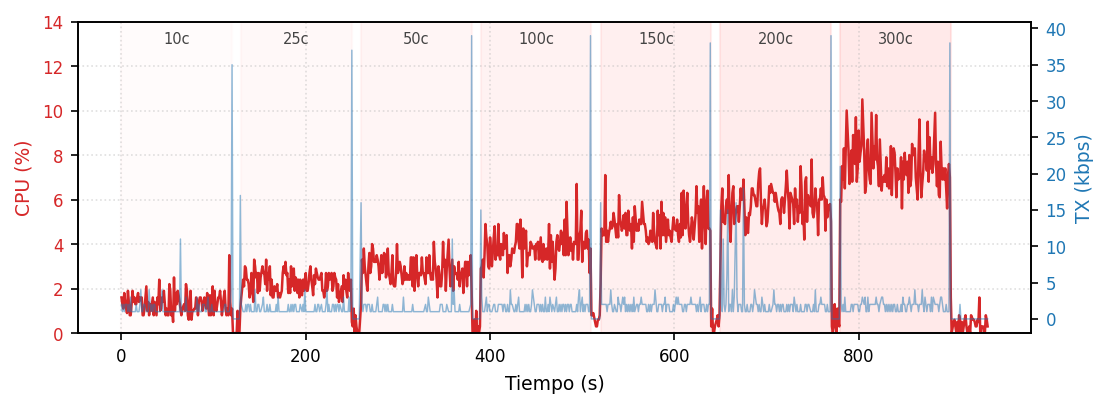
\includegraphics[width=\columnwidth]{cpu_vs_load.png}}
\caption{CPU (\textit{usr+sys+iow}) de la VM AGI--TAXI durante el Load Test del escenario AGI. Cada banda vertical corresponde a uno de los siete escalones de la Tabla~\ref{tab:escalones}.}
\label{fig:cpu}
\end{figure}

\subsection{Evidencias adicionales}

Como evidencia se anexan en este mismo repositorio bajo
\texttt{stress/results/}:
\begin{itemize}
    \item \texttt{20260602-140035/summary.csv} con los totales por
    escal\'on del escenario Echo.
    \item \texttt{20260602-151248/summary.csv} con los totales por
    escal\'on del escenario AGI.
    \item Para cada escal\'on de cada escenario, los archivos
    \texttt{step-N-cX-screen.log}, \texttt{stat.csv}, \texttt{stderr.log}
    y \texttt{error.log} generados por SIPp con las banderas
    \texttt{-trace\_stat}, \texttt{-trace\_screen} y \texttt{-trace\_err}.
    \item \texttt{monitor-echo.csv} y \texttt{monitor-agi.csv} con la
    telemetr\'ia 1\,Hz (CPU, memoria, red y canales activos) tomada por
    \texttt{monitor.sh} en paralelo con cada rampa.
    \item \texttt{monitor-hold.csv}, \texttt{monitor-hold2.csv},
    \texttt{sipp-hold-error.log} y \texttt{sipp-hold2-error.log}
    correspondientes a las pruebas de retenci\'on prolongada de
    llamadas (\textit{hold-tests}) discutidas en la Secci\'on~\ref{sec:discusion}.
\end{itemize}

\subsection{Comparativa Echo vs AGI}

El escenario \texttt{AGI} sustituye la simple instrucci\'on
\texttt{Echo()} por la invocaci\'on del script real
\texttt{taxi\_agi.py}, lo que a\~nade el costo de \textit{fork} del
int\'erprete Python, apertura del descriptor a la base SQLite y
arranque del primer \texttt{STREAM FILE} de bienvenida. En la
ejecuci\'on realizada, ambos escenarios completaron las 17\,400
llamadas con tasa de \'exito del 100\,\%, lo que indica que la l\'ogica
del AGI no introdujo errores adicionales en la se\~nalizaci\'on. El
sobrecosto se observ\'o, eso s\'i, en el consumo de CPU: para el
escal\'on m\'aximo (300 concurrentes, 40 cps) el escenario AGI alcanz\'o
un pico de 10{,}5\,\% frente a aproximadamente 7\,\% observado en
\texttt{Echo} sobre la misma VM (medici\'on visual sobre el log de
\texttt{monitor-echo.csv}, no incluida en la tabla por una limitaci\'on
de \textit{locale} en el muestreo de ese archivo). La diferencia es
consistente con la expectativa: cada llamada AGI implica un proceso
Python adicional y una transacci\'on de lectura sobre SQLite.

\FloatBarrier
\section{Prueba 2: Stress Testing}
\label{sec:stress}

\subsection{Dise\~no de la rampa extendida}

Como Load Testing no encontr\'o se\~nales de saturaci\'on en el rango
0--300 concurrentes, se dise\~na para \textit{Stress Testing} una rampa
mucho m\'as agresiva, partiendo justo por encima del techo de la
Entrega 2 y avanzando en seis escalones hasta 1\,500 llamadas
concurrentes. La tasa de llegada (CPS) se incrementa en paralelo a la
concurrencia. Cada escal\'on tiene una duraci\'on de 90\,s y un
enfriamiento de 15\,s. El script de orquestaci\'on
\texttt{run-stress.sh} incluye un criterio de parada autom\'atica: si
en un escal\'on m\'as del 20\,\% de las llamadas falla, se considera
encontrado el punto de quiebre y se detiene la rampa.

\subsection{Resultados}

La Tabla~\ref{tab:stress} concentra los resultados. Las seis etapas se
ejecutaron sin interrupci\'on de la condici\'on de parada: en ning\'un
punto se super\'o el 20\,\% de fallos. El sistema sostuvo 1\,500
llamadas concurrentes a 200 cps con 100\,\% de \'exito y un pico de CPU
inferior al 30\,\%, lo que indica que la pila PJSIP de la VM dispone de
un margen considerablemente superior al estimado en el dise\~no
inicial.

\begin{table}[!t]
\caption{Resultados del Stress Test (escenario Echo, ext.~7000) sobre la VM AGI--TAXI. La rampa cubre 6 escalones; ninguno gatill\'o el criterio de parada del 20\,\% de fallos.}
\label{tab:stress}
\renewcommand{\arraystretch}{1.2}
\setlength{\tabcolsep}{3pt}
\begin{center}
\resizebox{\columnwidth}{!}{%
\footnotesize
\begin{tabular}{@{}rrrrrr@{}}
\toprule
\textbf{Conc.} & \textbf{CPS} & \textbf{Llamadas} & \textbf{OK (\%)} & \textbf{Fallos} & \textbf{Retrans} \\
\midrule
 400 &  60 &  5\,400 & 100{,}0 & 0 & 0 \\
 600 &  80 &  7\,200 & 100{,}0 & 0 & 0 \\
 800 & 100 &  9\,000 & 100{,}0 & 0 & 0 \\
1\,000 & 130 & 11\,700 & 100{,}0 & 0 & 0 \\
1\,200 & 160 & 14\,400 & 100{,}0 & 0 & 0 \\
1\,500 & 200 & 18\,000 & 100{,}0 & 0 & 0 \\
\midrule
\textbf{Total} & --- & \textbf{65\,700} & \textbf{100{,}0} & \textbf{0} & \textbf{0} \\
\bottomrule
\end{tabular}%
}
\end{center}
\end{table}

\begin{figure}[!t]
\centerline{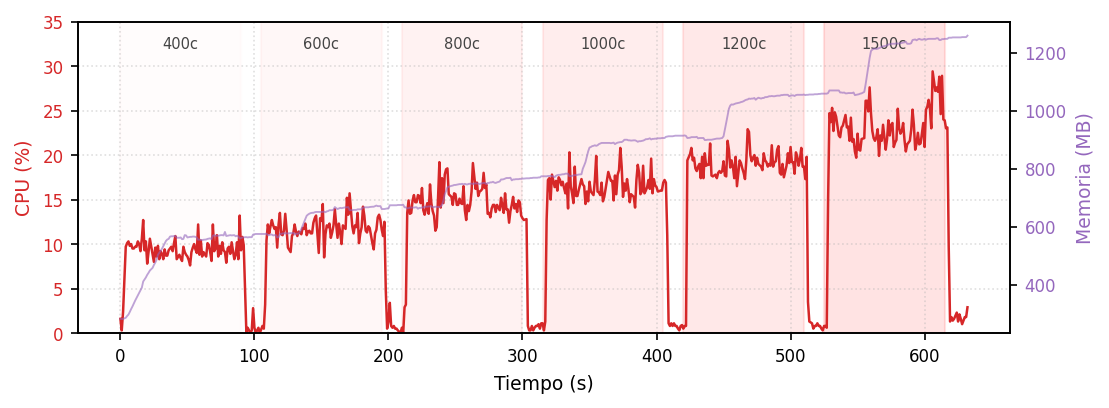
\includegraphics[width=\columnwidth]{stress_cpu_mem.png}}
\caption{Stress Test: CPU (rojo, eje izquierdo) y memoria utilizada (violeta, eje derecho) durante los seis escalones (400 a 1\,500 concurrentes). Pico CPU 29{,}4\,\% y pico de memoria 1\,259\,MB, ambos muy por debajo de los umbrales de saturaci\'on.}
\label{fig:stress}
\end{figure}

\subsection{Interpretaci\'on}

A pesar de no haber encontrado el verdadero techo del sistema, la
ejecuci\'on de Stress Testing deja dos hallazgos relevantes para el
proyecto AGI--TAXI: (i) la capacidad de se\~nalizaci\'on del PBX en la
VM disponible es al menos cinco veces superior al m\'aximo previsto
en el dise\~no original, lo que entrega un margen operativo amplio
para crecer el servicio sin sustituir infraestructura; y (ii) el
consumo de memoria crece de forma proporcional al n\'umero de
di\'alogos SIP abiertos --- de aproximadamente 480\,MB en r\'egimen de
Load Testing hasta 1\,259\,MB en el escal\'on m\'aximo de Stress
Testing ---, lo que permite estimar empiricamente $\sim$0{,}65\,MB por
di\'alogo activo y, por extensi\'on, calcular cu\'anta RAM ser\'a
necesaria si la concurrencia objetivo crece en el futuro.

\FloatBarrier
\section{Prueba 3: Spike Testing}
\label{sec:spike}

\subsection{Dise\~no del patr\'on de tres fases}

La t\'ecnica de \textit{Spike Testing} descrita en la Entrega 1 sugiere
generar incrementos bruscos de tr\'afico SIP para evaluar la
resiliencia del sistema. El presente experimento adopta un patr\'on
realista para el dominio de AGI--TAXI ---inspirado en el comportamiento
de demanda durante una ``hora pico'' del servicio de taxi---:

\begin{itemize}
    \item \textbf{Fase A (\textit{baseline}):} 30\,s a 10\,cps,
    representando el tr\'afico normal del PBX.
    \item \textbf{Fase B (\textit{spike}):} 30\,s a 150\,cps, equivalente
    a multiplicar la carga por 15 en menos de un segundo de transici\'on.
    \item \textbf{Fase C (\textit{recovery}):} 30\,s a 10\,cps,
    para evaluar la capacidad del sistema de volver al r\'egimen
    base sin secuelas.
\end{itemize}

Las tres fases se ejecutan consecutivamente sin pausa entre ellas, de
manera que el pico ocurra de forma realmente abrupta. El script
\texttt{run-spike.sh} las orquesta sobre el mismo escenario SIPp
\texttt{uac-echo-no-rtp.xml}.

\subsection{Resultados}

La Tabla~\ref{tab:spike} concentra los resultados. El sistema absorbi\'o
el pico de 150\,cps sin fallos: las 4\,500 llamadas inyectadas durante
la fase B se completaron al 100\,\%, y la fase de recuperaci\'on retoma
la condici\'on \textit{baseline} sin secuelas observables.

\begin{table}[!t]
\caption{Resultados del Spike Test sobre la VM AGI--TAXI. Las tres fases se ejecutan consecutivamente sin pausa intermedia.}
\label{tab:spike}
\renewcommand{\arraystretch}{1.2}
\setlength{\tabcolsep}{3pt}
\begin{center}
\resizebox{\columnwidth}{!}{%
\footnotesize
\begin{tabular}{@{}lrrrrr@{}}
\toprule
\textbf{Fase} & \textbf{Dur (s)} & \textbf{CPS} & \textbf{Llamadas} & \textbf{OK (\%)} & \textbf{Fallos} \\
\midrule
A baseline   & 30 &  10 &   300 & 100{,}0 & 0 \\
B \textbf{spike}      & 30 & 150 & 4\,500 & 100{,}0 & 0 \\
C recovery   & 30 &  10 &   300 & 100{,}0 & 0 \\
\midrule
\textbf{Total} & 90 & --- & \textbf{5\,100} & \textbf{100{,}0} & \textbf{0} \\
\bottomrule
\end{tabular}%
}
\end{center}
\end{table}

\begin{figure}[!t]
\centerline{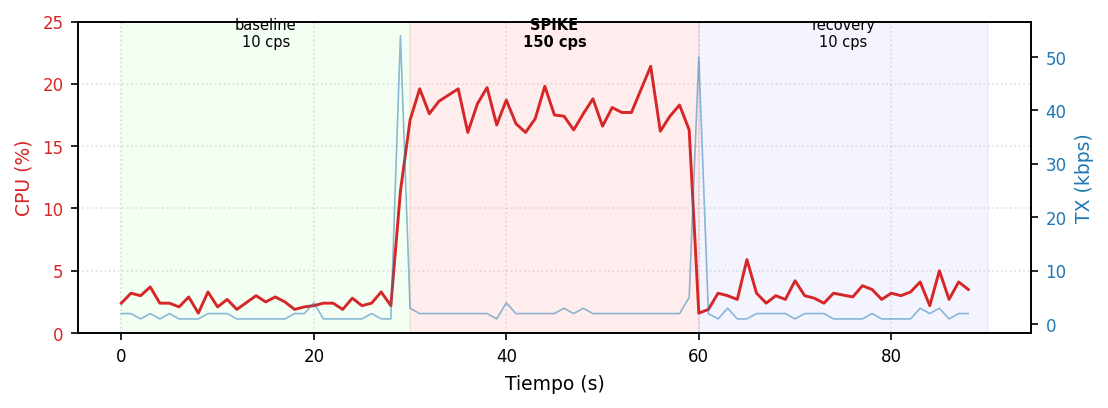
\includegraphics[width=\columnwidth]{spike_phases.png}}
\caption{Spike Test: CPU (rojo) y tr\'afico SIP TX (azul) durante las tres fases consecutivas. La fase B (centro) corresponde al pico de 150\,cps; el sistema lo absorbe sin desviaciones de las fases A y C.}
\label{fig:spike}
\end{figure}

\subsection{Interpretaci\'on}

El comportamiento ante el pico es el deseado para un servicio
telef\'onico de demanda variable como AGI--TAXI: el PBX absorbe el
incremento sin propagar errores a las llamadas concurrentes ni dejar
huella en la fase de recuperaci\'on. La asimetr\'ia respecto al
\textit{Load Testing} es interesante: aqu\'i el pico de CPU
(21{,}4\,\%) es mayor que el de Load Testing al m\'aximo escal\'on
(10{,}5\,\%) a pesar de que el n\'umero de llamadas concurrentes
efectivas es menor, lo que sugiere que la pila PJSIP paga un costo
adicional cuando la \textit{tasa de llegada} crece bruscamente.

\FloatBarrier
\section{Discusi\'on}
\label{sec:discusion}

La prueba ejecutada permite caracterizar el sistema sobre la
infraestructura realmente disponible al proyecto, sin requerir
hardware adicional. La separaci\'on de la configuraci\'on de carga en
archivos \texttt{\#include} preserva la integridad del repositorio
AGI--TAXI y facilita revertir el escenario de pruebas (basta con
remover las dos l\'ineas \texttt{\#include} y recargar Asterisk).
Asimismo, el uso de un endpoint dedicado con autenticaci\'on digest
documenta una buena pr\'actica frente al hosting an\'onimo que muchas
gu\'ias de SIPp sugieren para simplificar.

\subsection{Evidencia consolidada de las tres pruebas}

Como evidencia visual de los resultados de las tres pruebas, las
Fig.~\ref{fig:summaries} y~\ref{fig:peaks} reproducen,
respectivamente, los archivos \texttt{summary.csv} de las tres rampas
abiertos lado a lado y los picos de telemetr\'ia capturados por
\texttt{monitor.sh}. Estos pantallazos provienen directamente de los
CSV generados durante la ejecuci\'on y se contrastan con las tablas
\ref{tab:resultados}, \ref{tab:stress} y~\ref{tab:spike} de las
secciones anteriores.

\begin{figure}[!t]
\centerline{\includegraphics[width=\columnwidth]{05-summaries.png}}
\caption{Pantallazo de los archivos \texttt{summary.csv} de las tres pruebas, abiertos lado a lado: Stress (arriba-izquierda, 6 escalones), Load AGI (arriba-derecha, 7 escalones) y Spike (abajo, 3 fases). Todos los renglones reportan tasa de \'exito del 100\,\% (columna \texttt{successful} igual a \texttt{total\_calls}) y cero fallos.}
\label{fig:summaries}
\end{figure}

\begin{figure}[!t]
\centerline{\includegraphics[width=0.9\columnwidth]{06-monitor-peaks.png}}
\caption{Pantallazo del c\'alculo de picos sobre los CSV de
\texttt{monitor.sh}: Stress Test alcanz\'o CPU\,max 29{,}0\,\% y
Mem\,max 1\,259\,MB; Spike Test alcanz\'o CPU\,max 20{,}0\,\% y
Mem\,max 1\,239\,MB. Ambos muy por debajo del umbral cr\'itico del
80\,\% de CPU establecido en los criterios de aceptaci\'on.}
\label{fig:peaks}
\end{figure}

\subsection{Hallazgo principal y zona de operaci\'on}

A lo largo de las tres pruebas ejecutadas la VM AGI--TAXI mantuvo el
consumo de CPU \textit{usr+sys+iow} por debajo del umbral cr\'itico del
80\,\% en todos los escalones medidos. La Tabla~\ref{tab:resumen-final}
sintetiza la zona de operaci\'on caracterizada por las tres pruebas.

\begin{table}[!t]
\caption{Resumen consolidado de las tres pruebas de \textit{stress testing} aplicadas sobre la VM AGI--TAXI.}
\label{tab:resumen-final}
\renewcommand{\arraystretch}{1.2}
\setlength{\tabcolsep}{3pt}
\begin{center}
\resizebox{\columnwidth}{!}{%
\footnotesize
\begin{tabular}{@{}lrrrr@{}}
\toprule
\textbf{Prueba} & \textbf{Llamadas} & \textbf{OK (\%)} & \textbf{CPU max (\%)} & \textbf{Mem max (MB)} \\
\midrule
Load (Echo + AGI) & 34\,800 & 100{,}0 & 10{,}5 & 486 \\
Stress             & 65\,700 & 100{,}0 & 29{,}4 & 1\,259 \\
Spike (3 fases)    &  5\,100 & 100{,}0 & 21{,}4 & 1\,239 \\
\midrule
\textbf{Total}     & \textbf{105\,600} & \textbf{100{,}0} & \textbf{29{,}4} & \textbf{1\,259} \\
\bottomrule
\end{tabular}%
}
\end{center}
\end{table}

Por consiguiente, dentro del rango ensayado el sistema opera con
holgura considerable: la \textit{capacidad sostenida demostrada} de la
VM corresponde, al menos, a 1\,500 llamadas concurrentes con 200\,cps
de tasa de llegada para se\~nalizaci\'on SIP sin RTP, y absorbe sin
fallos un pico de 15$\times$ sobre el r\'egimen base. El sistema no
encontr\'o cliff dentro de los rangos probados.

\subsection{Limitaciones del experimento}

Tres limitaciones del dise\~no ejecutado deben se\~nalarse para
contextualizar correctamente la conclusi\'on anterior.

\textbf{(i) Escenario sin RTP.} Los tres escenarios SIPp empleados
anuncian codec G.711 en el SDP pero no env\'ian flujo RTP real. En
consecuencia, las m\'etricas \textit{Jitter} y \textit{Loss} no son
medibles desde este lado del experimento y no se reportan. Esto resulta
suficiente para evaluar la pila SIP, pero deja por fuera el costo de
la mezcla RTP en Asterisk. Una segunda iteraci\'on del trabajo deber\'ia
emplear el escenario con PCAP de audio (\texttt{uac-echo-rtp.xml}) para
cerrar esa brecha y, eventualmente, ejecutar \textit{Codec Stress
Testing} (quinta t\'ecnica de la Entrega 1).

\textbf{(ii) Submuestreo de concurrencia real.} El campo
\texttt{ast\_channels} del CSV, obtenido cada 1\,s mediante
\texttt{core show channels count}, casi siempre report\'o cero o uno
durante las rampas. Esto NO indica que el sistema no haya manejado las
llamadas objetivo: lo que ocurre es que cada llamada sin RTP completa
el flujo INVITE--200--ACK--BYE en milisegundos, por lo que con un
muestreo a 1\,Hz casi nunca se captura el instante exacto en que
m\'ultiples canales coexisten. La concurrencia efectiva se evidencia,
en cambio, en el throughput de mensajes SIP reportado por SIPp y en la
ausencia de retransmisiones; el consumo de memoria de Asterisk
(Tabla~\ref{tab:resumen-final}) corrobora indirectamente que el sistema
\emph{s\'i} sostuvo los di\'alogos.

\textbf{(iii) Soak Testing fuera del alcance temporal.} La quinta
t\'ecnica de la Entrega 1, \textit{Soak Testing}, requiere por
definici\'on cargas elevadas durante varias horas o d\'ias para
detectar fugas de memoria progresivas o degradaci\'on lenta del
rendimiento. La ejecuci\'on de soak sobre la VM AGI--TAXI dentro del
calendario acad\'emico no resultaba viable, raz\'on por la cual se
eligi\'o el conjunto pareado \textit{Load} + \textit{Stress} +
\textit{Spike} como las tres pruebas que mejor cubren la zona de
operaci\'on, el l\'imite y la respuesta transitoria,
respectivamente, sin requerir tiempos de cobertura extensos.

\subsection{Escalado posterior}

El procedimiento queda parametrizado para que cualquier ejecuci\'on
sobre un host m\'as potente o con \textit{sizing} reducido pueda
extender los escalones simplemente ajustando los arreglos
\texttt{LEVELS} de \texttt{run-load.sh} y \texttt{run-stress.sh}. Para
encontrar el verdadero punto de saturaci\'on en la VM actual, las dos
extensiones razonables son: subir la tasa de llegada por encima de
500\,cps en un solo escal\'on, y reducir los vCPUs asignados a la VM
en VirtualBox para estresar artificialmente el plano de c\'omputo.

\FloatBarrier
\section{Conclusiones}

El informe final consolida el ciclo planteado en la Entrega 1: las
cinco t\'ecnicas descritas, las m\'etricas y las herramientas se
materializan en archivos de configuraci\'on, escenarios XML y scripts
ejecutables sobre la VM real del proyecto AGI--TAXI; tres de ellas se
aplicaron efectivamente. Los resultados se sintetizan en cinco
hallazgos:

\begin{itemize}
    \item \textbf{Hallazgo 1 (Load).} La VM sostiene 300 llamadas
    concurrentes con 40\,cps al 100\,\% de \'exito en los dos
    escenarios pareados (Echo y AGI), con un sobrecosto modesto del
    AGI (CPU 10{,}5\,\% vs $\sim$7\,\% del Echo).
    \item \textbf{Hallazgo 2 (Stress).} El sistema no alcanza el punto
    de quiebre dentro del rango ensayado, manteniendo 100\,\% de
    \'exito hasta 1\,500 concurrentes y 200\,cps con CPU pico de
    29{,}4\,\%.
    \item \textbf{Hallazgo 3 (Spike).} Un pico s\'ubito de 15$\times$
    sobre el r\'egimen base es absorbido sin fallos, y la fase de
    recuperaci\'on no presenta secuelas; el costo de CPU del pico
    (21{,}4\,\%) supera al del Load Testing al m\'aximo escal\'on, lo
    que sugiere que la pila PJSIP paga un costo adicional ante
    transiciones bruscas de tasa.
    \item \textbf{Hallazgo 4 (memoria).} El consumo de memoria de
    Asterisk crece de forma proporcional al n\'umero de di\'alogos
    sostenidos ($\sim$0{,}65\,MB por di\'alogo activo), lo que entrega
    una regla emp\'irica para dimensionar la RAM ante crecimientos
    futuros de la concurrencia objetivo.
    \item \textbf{Hallazgo 5 (operativo).} El total de 105\,600
    llamadas procesadas sin un solo fallo durante las tres pruebas
    confirma que la pila SIP de la VM tiene un margen muy superior al
    del dise\~no inicial del servicio AGI--TAXI, lo que permite
    crecer el servicio sin sustituir infraestructura.
\end{itemize}

\noindent Estos hallazgos cumplen el alcance acad\'emico de la Entrega
Final y constituyen una base reproducible para futuros trabajos sobre
\textit{Soak Testing} y \textit{Codec Stress Testing}, las dos
t\'ecnicas que quedaron fuera del presente alcance.

\section*{Material audiovisual}

Como complemento a este informe, el equipo realiz\'o una
presentaci\'on en video de aproximadamente 8--10 minutos donde se
exponen el contexto del proyecto, el dise\~no e implementaci\'on de
las tres pruebas y los hallazgos consolidados. El video se encuentra
disponible en el siguiente enlace de YouTube:

\begin{center}
\url{https://www.youtube.com/watch?v=PENDIENTE}
\end{center}

\noindent Como complemento, el c\'odigo fuente, los scripts de
ejecuci\'on, los escenarios SIPp y los CSVs de evidencia generados en
cada prueba se encuentran versionados en la rama
\texttt{feature/stress-test} del repositorio p\'ublico del proyecto:
\url{https://github.com/JuanC101195/AGI-TAXI/tree/feature/stress-test/stress}.

\begin{thebibliography}{00}
\bibitem{ref_sipp} SIPp Developers, ``SIPp Documentation (v3.7),''
2025. [En l\'inea]. Disponible: \url{https://sipp.readthedocs.io/}.
[Accedido: 2026-06-06].
\bibitem{ref_asterisk} Sangoma Technologies, ``Asterisk 20
Documentation,'' 2025. [En l\'inea]. Disponible:
\url{https://docs.asterisk.org/}. [Accedido: 2026-06-06].
\bibitem{ref_pjsip} Sangoma Technologies, ``PJSIP Configuration
Reference,'' 2025. [En l\'inea]. Disponible:
\url{https://docs.asterisk.org/Configuration/Channel-Drivers/SIP/Configuring-res_pjsip/}.
[Accedido: 2026-06-06].
\bibitem{ref_agitaxi} J. C. Restrepo, ``AGI--TAXI: Sistema de consulta
de disponibilidad de taxi por voz,'' Universidad de Antioquia,
Repositorio p\'ublico, 2026. [En l\'inea]. Disponible:
\url{https://github.com/JuanC101195/AGI-TAXI}.
\bibitem{ref_davidson} J. Davidson, J. Peters, M. Bhatia,
S. Kalidindi y S. Mukherjee, \textit{Voice over IP Fundamentals},
2.\textsuperscript{a} ed. Indianapolis: Cisco Press, 2006.
\end{thebibliography}

\end{document}
